% Options for packages loaded elsewhere
\PassOptionsToPackage{unicode}{hyperref}
\PassOptionsToPackage{hyphens}{url}
%
\documentclass[
]{article}
\usepackage{lmodern}
\usepackage{amssymb,amsmath}
\usepackage{ifxetex,ifluatex}
\ifnum 0\ifxetex 1\fi\ifluatex 1\fi=0 % if pdftex
  \usepackage[T1]{fontenc}
  \usepackage[utf8]{inputenc}
  \usepackage{textcomp} % provide euro and other symbols
\else % if luatex or xetex
  \usepackage{unicode-math}
  \defaultfontfeatures{Scale=MatchLowercase}
  \defaultfontfeatures[\rmfamily]{Ligatures=TeX,Scale=1}
\fi
% Use upquote if available, for straight quotes in verbatim environments
\IfFileExists{upquote.sty}{\usepackage{upquote}}{}
\IfFileExists{microtype.sty}{% use microtype if available
  \usepackage[]{microtype}
  \UseMicrotypeSet[protrusion]{basicmath} % disable protrusion for tt fonts
}{}
\makeatletter
\@ifundefined{KOMAClassName}{% if non-KOMA class
  \IfFileExists{parskip.sty}{%
    \usepackage{parskip}
  }{% else
    \setlength{\parindent}{0pt}
    \setlength{\parskip}{6pt plus 2pt minus 1pt}}
}{% if KOMA class
  \KOMAoptions{parskip=half}}
\makeatother
\usepackage{xcolor}
\IfFileExists{xurl.sty}{\usepackage{xurl}}{} % add URL line breaks if available
\IfFileExists{bookmark.sty}{\usepackage{bookmark}}{\usepackage{hyperref}}
\hypersetup{
  pdftitle={Updated Report for Edovo 8-5},
  pdfauthor={Abby Smith},
  hidelinks,
  pdfcreator={LaTeX via pandoc}}
\urlstyle{same} % disable monospaced font for URLs
\usepackage[margin=1in]{geometry}
\usepackage{longtable,booktabs}
% Correct order of tables after \paragraph or \subparagraph
\usepackage{etoolbox}
\makeatletter
\patchcmd\longtable{\par}{\if@noskipsec\mbox{}\fi\par}{}{}
\makeatother
% Allow footnotes in longtable head/foot
\IfFileExists{footnotehyper.sty}{\usepackage{footnotehyper}}{\usepackage{footnote}}
\makesavenoteenv{longtable}
\usepackage{graphicx,grffile}
\makeatletter
\def\maxwidth{\ifdim\Gin@nat@width>\linewidth\linewidth\else\Gin@nat@width\fi}
\def\maxheight{\ifdim\Gin@nat@height>\textheight\textheight\else\Gin@nat@height\fi}
\makeatother
% Scale images if necessary, so that they will not overflow the page
% margins by default, and it is still possible to overwrite the defaults
% using explicit options in \includegraphics[width, height, ...]{}
\setkeys{Gin}{width=\maxwidth,height=\maxheight,keepaspectratio}
% Set default figure placement to htbp
\makeatletter
\def\fps@figure{htbp}
\makeatother
\setlength{\emergencystretch}{3em} % prevent overfull lines
\providecommand{\tightlist}{%
  \setlength{\itemsep}{0pt}\setlength{\parskip}{0pt}}
\setcounter{secnumdepth}{-\maxdimen} % remove section numbering

\title{Updated Report for Edovo 8-5}
\author{Abby Smith}
\date{8/5/2020}

\begin{document}
\maketitle

\begin{longtable}[]{@{}ll@{}}
\caption{Data summary}\tabularnewline
\toprule
\endhead
Name & edovo\_user\_data\tabularnewline
Number of rows & 288777\tabularnewline
Number of columns & 26\tabularnewline
\_\_\_\_\_\_\_\_\_\_\_\_\_\_\_\_\_\_\_\_\_\_\_ &\tabularnewline
Column type frequency: &\tabularnewline
character & 14\tabularnewline
Date & 1\tabularnewline
numeric & 8\tabularnewline
POSIXct & 3\tabularnewline
\_\_\_\_\_\_\_\_\_\_\_\_\_\_\_\_\_\_\_\_\_\_\_\_ &\tabularnewline
Group variables & None\tabularnewline
\bottomrule
\end{longtable}

\textbf{Variable type: character}

\begin{longtable}[]{@{}lrrrrrrr@{}}
\toprule
skim\_variable & n\_missing & complete\_rate & min & max & empty &
n\_unique & whitespace\tabularnewline
\midrule
\endhead
inmate\_id & 2 & 1.00 & 1 & 40 & 0 & 260099 & 0\tabularnewline
first\_name & 11431 & 0.96 & 1 & 31 & 0 & 48663 & 0\tabularnewline
last\_name & 11431 & 0.96 & 1 & 39 & 0 & 69006 & 0\tabularnewline
hashed\_password & 0 & 1.00 & 32 & 32 & 0 & 212918 & 0\tabularnewline
security\_question\_1 & 14096 & 0.95 & 14 & 128 & 0 & 2209 &
0\tabularnewline
security\_answer\_1 & 14088 & 0.95 & 1 & 128 & 0 & 102167 &
0\tabularnewline
security\_question\_2 & 14553 & 0.95 & 14 & 128 & 0 & 2209 &
0\tabularnewline
security\_answer\_2 & 14545 & 0.95 & 1 & 246 & 0 & 94689 &
0\tabularnewline
status & 0 & 1.00 & 6 & 11 & 0 & 4 & 0\tabularnewline
language & 0 & 1.00 & 5 & 5 & 0 & 2 & 0\tabularnewline
email & 265109 & 0.08 & 7 & 255 & 0 & 23309 & 0\tabularnewline
phone\_number & 268257 & 0.07 & 10 & 14 & 0 & 19909 & 0\tabularnewline
deactivation\_reason & 53557 & 0.81 & 1 & 431 & 0 & 2349 &
0\tabularnewline
zendesk\_id & 230605 & 0.20 & 30 & 34 & 0 & 58172 & 0\tabularnewline
\bottomrule
\end{longtable}

\textbf{Variable type: Date}

\begin{longtable}[]{@{}lrrlllr@{}}
\toprule
skim\_variable & n\_missing & complete\_rate & min & max & median &
n\_unique\tabularnewline
\midrule
\endhead
birth\_date & 0 & 1 & 0972-01-10 & 2020-07-24 & 1987-06-29 &
22986\tabularnewline
\bottomrule
\end{longtable}

\textbf{Variable type: numeric}

\begin{longtable}[]{@{}lrrrrrrrrrl@{}}
\toprule
\begin{minipage}[b]{0.08\columnwidth}\raggedright
skim\_variable\strut
\end{minipage} & \begin{minipage}[b]{0.04\columnwidth}\raggedleft
n\_missing\strut
\end{minipage} & \begin{minipage}[b]{0.06\columnwidth}\raggedleft
complete\_rate\strut
\end{minipage} & \begin{minipage}[b]{0.05\columnwidth}\raggedleft
mean\strut
\end{minipage} & \begin{minipage}[b]{0.05\columnwidth}\raggedleft
sd\strut
\end{minipage} & \begin{minipage}[b]{0.05\columnwidth}\raggedleft
p0\strut
\end{minipage} & \begin{minipage}[b]{0.05\columnwidth}\raggedleft
p25\strut
\end{minipage} & \begin{minipage}[b]{0.05\columnwidth}\raggedleft
p50\strut
\end{minipage} & \begin{minipage}[b]{0.05\columnwidth}\raggedleft
p75\strut
\end{minipage} & \begin{minipage}[b]{0.04\columnwidth}\raggedleft
p100\strut
\end{minipage} & \begin{minipage}[b]{0.17\columnwidth}\raggedright
hist\strut
\end{minipage}\tabularnewline
\midrule
\endhead
\begin{minipage}[t]{0.08\columnwidth}\raggedright
id\strut
\end{minipage} & \begin{minipage}[t]{0.04\columnwidth}\raggedleft
0\strut
\end{minipage} & \begin{minipage}[t]{0.06\columnwidth}\raggedleft
1.00\strut
\end{minipage} & \begin{minipage}[t]{0.05\columnwidth}\raggedleft
328850.24\strut
\end{minipage} & \begin{minipage}[t]{0.05\columnwidth}\raggedleft
153074.82\strut
\end{minipage} & \begin{minipage}[t]{0.05\columnwidth}\raggedleft
1.00\strut
\end{minipage} & \begin{minipage}[t]{0.05\columnwidth}\raggedleft
208060.00\strut
\end{minipage} & \begin{minipage}[t]{0.05\columnwidth}\raggedleft
380626.00\strut
\end{minipage} & \begin{minipage}[t]{0.05\columnwidth}\raggedleft
452853.00\strut
\end{minipage} & \begin{minipage}[t]{0.04\columnwidth}\raggedleft
525096\strut
\end{minipage} & \begin{minipage}[t]{0.17\columnwidth}\raggedright
▃▂▂▆▇\strut
\end{minipage}\tabularnewline
\begin{minipage}[t]{0.08\columnwidth}\raggedright
points\strut
\end{minipage} & \begin{minipage}[t]{0.04\columnwidth}\raggedleft
0\strut
\end{minipage} & \begin{minipage}[t]{0.06\columnwidth}\raggedleft
1.00\strut
\end{minipage} & \begin{minipage}[t]{0.05\columnwidth}\raggedleft
2724.22\strut
\end{minipage} & \begin{minipage}[t]{0.05\columnwidth}\raggedleft
222687.19\strut
\end{minipage} & \begin{minipage}[t]{0.05\columnwidth}\raggedleft
-186.25\strut
\end{minipage} & \begin{minipage}[t]{0.05\columnwidth}\raggedleft
14.67\strut
\end{minipage} & \begin{minipage}[t]{0.05\columnwidth}\raggedleft
38.56\strut
\end{minipage} & \begin{minipage}[t]{0.05\columnwidth}\raggedleft
213.24\strut
\end{minipage} & \begin{minipage}[t]{0.04\columnwidth}\raggedleft
100015006\strut
\end{minipage} & \begin{minipage}[t]{0.17\columnwidth}\raggedright
▇▁▁▁▁\strut
\end{minipage}\tabularnewline
\begin{minipage}[t]{0.08\columnwidth}\raggedright
total\_points\strut
\end{minipage} & \begin{minipage}[t]{0.04\columnwidth}\raggedleft
0\strut
\end{minipage} & \begin{minipage}[t]{0.06\columnwidth}\raggedleft
1.00\strut
\end{minipage} & \begin{minipage}[t]{0.05\columnwidth}\raggedleft
40369.77\strut
\end{minipage} & \begin{minipage}[t]{0.05\columnwidth}\raggedleft
4748704.98\strut
\end{minipage} & \begin{minipage}[t]{0.05\columnwidth}\raggedleft
0.00\strut
\end{minipage} & \begin{minipage}[t]{0.05\columnwidth}\raggedleft
0.25\strut
\end{minipage} & \begin{minipage}[t]{0.05\columnwidth}\raggedleft
118.49\strut
\end{minipage} & \begin{minipage}[t]{0.05\columnwidth}\raggedleft
1648.11\strut
\end{minipage} & \begin{minipage}[t]{0.04\columnwidth}\raggedleft
931797121\strut
\end{minipage} & \begin{minipage}[t]{0.17\columnwidth}\raggedright
▇▁▁▁▁\strut
\end{minipage}\tabularnewline
\begin{minipage}[t]{0.08\columnwidth}\raggedright
total\_spent\_points\strut
\end{minipage} & \begin{minipage}[t]{0.04\columnwidth}\raggedleft
0\strut
\end{minipage} & \begin{minipage}[t]{0.06\columnwidth}\raggedleft
1.00\strut
\end{minipage} & \begin{minipage}[t]{0.05\columnwidth}\raggedleft
16998.57\strut
\end{minipage} & \begin{minipage}[t]{0.05\columnwidth}\raggedleft
2905728.04\strut
\end{minipage} & \begin{minipage}[t]{0.05\columnwidth}\raggedleft
0.00\strut
\end{minipage} & \begin{minipage}[t]{0.05\columnwidth}\raggedleft
0.00\strut
\end{minipage} & \begin{minipage}[t]{0.05\columnwidth}\raggedleft
89.89\strut
\end{minipage} & \begin{minipage}[t]{0.05\columnwidth}\raggedleft
1595.68\strut
\end{minipage} & \begin{minipage}[t]{0.04\columnwidth}\raggedleft
913471373\strut
\end{minipage} & \begin{minipage}[t]{0.17\columnwidth}\raggedright
▇▁▁▁▁\strut
\end{minipage}\tabularnewline
\begin{minipage}[t]{0.08\columnwidth}\raggedright
facility\_id\strut
\end{minipage} & \begin{minipage}[t]{0.04\columnwidth}\raggedleft
0\strut
\end{minipage} & \begin{minipage}[t]{0.06\columnwidth}\raggedleft
1.00\strut
\end{minipage} & \begin{minipage}[t]{0.05\columnwidth}\raggedleft
294.98\strut
\end{minipage} & \begin{minipage}[t]{0.05\columnwidth}\raggedleft
229.95\strut
\end{minipage} & \begin{minipage}[t]{0.05\columnwidth}\raggedleft
0.00\strut
\end{minipage} & \begin{minipage}[t]{0.05\columnwidth}\raggedleft
96.00\strut
\end{minipage} & \begin{minipage}[t]{0.05\columnwidth}\raggedleft
227.00\strut
\end{minipage} & \begin{minipage}[t]{0.05\columnwidth}\raggedleft
505.00\strut
\end{minipage} & \begin{minipage}[t]{0.04\columnwidth}\raggedleft
735\strut
\end{minipage} & \begin{minipage}[t]{0.17\columnwidth}\raggedright
▇▂▃▃▃\strut
\end{minipage}\tabularnewline
\begin{minipage}[t]{0.08\columnwidth}\raggedright
credit\_balance\strut
\end{minipage} & \begin{minipage}[t]{0.04\columnwidth}\raggedleft
0\strut
\end{minipage} & \begin{minipage}[t]{0.06\columnwidth}\raggedleft
1.00\strut
\end{minipage} & \begin{minipage}[t]{0.05\columnwidth}\raggedleft
0.00\strut
\end{minipage} & \begin{minipage}[t]{0.05\columnwidth}\raggedleft
0.06\strut
\end{minipage} & \begin{minipage}[t]{0.05\columnwidth}\raggedleft
0.00\strut
\end{minipage} & \begin{minipage}[t]{0.05\columnwidth}\raggedleft
0.00\strut
\end{minipage} & \begin{minipage}[t]{0.05\columnwidth}\raggedleft
0.00\strut
\end{minipage} & \begin{minipage}[t]{0.05\columnwidth}\raggedleft
0.00\strut
\end{minipage} & \begin{minipage}[t]{0.04\columnwidth}\raggedleft
31\strut
\end{minipage} & \begin{minipage}[t]{0.17\columnwidth}\raggedright
▇▁▁▁▁\strut
\end{minipage}\tabularnewline
\begin{minipage}[t]{0.08\columnwidth}\raggedright
balance\strut
\end{minipage} & \begin{minipage}[t]{0.04\columnwidth}\raggedleft
0\strut
\end{minipage} & \begin{minipage}[t]{0.06\columnwidth}\raggedleft
1.00\strut
\end{minipage} & \begin{minipage}[t]{0.05\columnwidth}\raggedleft
0.02\strut
\end{minipage} & \begin{minipage}[t]{0.05\columnwidth}\raggedleft
1.56\strut
\end{minipage} & \begin{minipage}[t]{0.05\columnwidth}\raggedleft
0.00\strut
\end{minipage} & \begin{minipage}[t]{0.05\columnwidth}\raggedleft
0.00\strut
\end{minipage} & \begin{minipage}[t]{0.05\columnwidth}\raggedleft
0.00\strut
\end{minipage} & \begin{minipage}[t]{0.05\columnwidth}\raggedleft
0.00\strut
\end{minipage} & \begin{minipage}[t]{0.04\columnwidth}\raggedleft
166\strut
\end{minipage} & \begin{minipage}[t]{0.17\columnwidth}\raggedright
▇▁▁▁▁\strut
\end{minipage}\tabularnewline
\begin{minipage}[t]{0.08\columnwidth}\raggedright
desk\_id\strut
\end{minipage} & \begin{minipage}[t]{0.04\columnwidth}\raggedleft
159502\strut
\end{minipage} & \begin{minipage}[t]{0.06\columnwidth}\raggedleft
0.45\strut
\end{minipage} & \begin{minipage}[t]{0.05\columnwidth}\raggedleft
642937403.52\strut
\end{minipage} & \begin{minipage}[t]{0.05\columnwidth}\raggedleft
100138448.17\strut
\end{minipage} & \begin{minipage}[t]{0.05\columnwidth}\raggedleft
267779098.00\strut
\end{minipage} & \begin{minipage}[t]{0.05\columnwidth}\raggedleft
583932457.00\strut
\end{minipage} & \begin{minipage}[t]{0.05\columnwidth}\raggedleft
675915499.00\strut
\end{minipage} & \begin{minipage}[t]{0.05\columnwidth}\raggedleft
723340111.50\strut
\end{minipage} & \begin{minipage}[t]{0.04\columnwidth}\raggedleft
757482999\strut
\end{minipage} & \begin{minipage}[t]{0.17\columnwidth}\raggedright
▁▁▂▃▇\strut
\end{minipage}\tabularnewline
\bottomrule
\end{longtable}

\textbf{Variable type: POSIXct}

\begin{longtable}[]{@{}lrrlllr@{}}
\toprule
\begin{minipage}[b]{0.11\columnwidth}\raggedright
skim\_variable\strut
\end{minipage} & \begin{minipage}[b]{0.08\columnwidth}\raggedleft
n\_missing\strut
\end{minipage} & \begin{minipage}[b]{0.11\columnwidth}\raggedleft
complete\_rate\strut
\end{minipage} & \begin{minipage}[b]{0.15\columnwidth}\raggedright
min\strut
\end{minipage} & \begin{minipage}[b]{0.15\columnwidth}\raggedright
max\strut
\end{minipage} & \begin{minipage}[b]{0.15\columnwidth}\raggedright
median\strut
\end{minipage} & \begin{minipage}[b]{0.07\columnwidth}\raggedleft
n\_unique\strut
\end{minipage}\tabularnewline
\midrule
\endhead
\begin{minipage}[t]{0.11\columnwidth}\raggedright
created\_at\strut
\end{minipage} & \begin{minipage}[t]{0.08\columnwidth}\raggedleft
0\strut
\end{minipage} & \begin{minipage}[t]{0.11\columnwidth}\raggedleft
1.00\strut
\end{minipage} & \begin{minipage}[t]{0.15\columnwidth}\raggedright
2014-04-16 01:37:58\strut
\end{minipage} & \begin{minipage}[t]{0.15\columnwidth}\raggedright
2020-07-27 16:43:44\strut
\end{minipage} & \begin{minipage}[t]{0.15\columnwidth}\raggedright
2019-01-25 18:08:56\strut
\end{minipage} & \begin{minipage}[t]{0.07\columnwidth}\raggedleft
288343\strut
\end{minipage}\tabularnewline
\begin{minipage}[t]{0.11\columnwidth}\raggedright
updated\_at\strut
\end{minipage} & \begin{minipage}[t]{0.08\columnwidth}\raggedleft
0\strut
\end{minipage} & \begin{minipage}[t]{0.11\columnwidth}\raggedleft
1.00\strut
\end{minipage} & \begin{minipage}[t]{0.15\columnwidth}\raggedright
2016-06-09 22:57:51\strut
\end{minipage} & \begin{minipage}[t]{0.15\columnwidth}\raggedright
2020-07-27 16:53:43\strut
\end{minipage} & \begin{minipage}[t]{0.15\columnwidth}\raggedright
2019-08-28 15:05:08\strut
\end{minipage} & \begin{minipage}[t]{0.07\columnwidth}\raggedleft
273538\strut
\end{minipage}\tabularnewline
\begin{minipage}[t]{0.11\columnwidth}\raggedright
release\_date\strut
\end{minipage} & \begin{minipage}[t]{0.08\columnwidth}\raggedleft
264923\strut
\end{minipage} & \begin{minipage}[t]{0.11\columnwidth}\raggedleft
0.08\strut
\end{minipage} & \begin{minipage}[t]{0.15\columnwidth}\raggedright
1902-05-14 00:00:00\strut
\end{minipage} & \begin{minipage}[t]{0.15\columnwidth}\raggedright
2099-12-31 00:00:00\strut
\end{minipage} & \begin{minipage}[t]{0.15\columnwidth}\raggedright
2019-12-29 00:00:00\strut
\end{minipage} & \begin{minipage}[t]{0.07\columnwidth}\raggedleft
3977\strut
\end{minipage}\tabularnewline
\bottomrule
\end{longtable}

\hypertarget{overall-duplication-rate}{%
\subsubsection{Overall Duplication
Rate}\label{overall-duplication-rate}}

\begin{verbatim}
## # A tibble: 1 x 1
##   percent_dup
##         <dbl>
## 1       0.275
\end{verbatim}

\hypertarget{for-each-clearly-duplicate-user-what-ids-are-they-using}{%
\subsubsection{\texorpdfstring{For each \textbf{clearly} duplicate user,
what IDs are they
using?}{For each clearly duplicate user, what IDs are they using?}}\label{for-each-clearly-duplicate-user-what-ids-are-they-using}}

\begin{verbatim}
## # A tibble: 29,623 x 3
## # Groups:   first_name [5,097]
##    first_name last_name id                                                      
##    <chr>      <chr>     <chr>                                                   
##  1 -          -         410052,405133,406993,383037,401380,401391,404485,401671~
##  2 --         --        397568,424721                                           
##  3 A          A         30596,30599,30602,59529,118811,98365,196936,196828,1960~
##  4 A          B         9365,68641,101476,84511,106910,123317,187321,169609,196~
##  5 A          C         511985,512521                                           
##  6 A          D         917,68632,75647,400077,400186,524589,520432,518167      
##  7 A          E         381358,464600                                           
##  8 A          F         386260,383781,517953                                    
##  9 A          G         75650,333802,365025                                     
## 10 A          J         5955,176125,359649,387507,388288,508865,508448,508785,5~
## # ... with 29,613 more rows
\end{verbatim}

\hypertarget{for-each-clearly-duplicate-user-how-do-the-points-stack-up-across-accounts}{%
\subsubsection{\texorpdfstring{For each \textbf{clearly} duplicate user:
How do the points stack up across
accounts?}{For each clearly duplicate user: How do the points stack up across accounts?}}\label{for-each-clearly-duplicate-user-how-do-the-points-stack-up-across-accounts}}

\begin{verbatim}
## # A tibble: 29,623 x 3
## # Groups:   first_name [5,097]
##    first_name last_name sum_points
##    <chr>      <chr>          <dbl>
##  1 Michael    Sharp     931797121.
##  2 Jose       Padilla   772534473.
##  3 Jason      Wood      696262753.
##  4 Terry      Person    695472135 
##  5 George     Varela    209043083.
##  6 Jessica    Hernandez 122750203.
##  7 James      Burke     107338135.
##  8 Darren     Thompson   48445889.
##  9 Brian      Combs      22060020.
## 10 Jason      Young      17827854.
## # ... with 29,613 more rows
\end{verbatim}

\hypertarget{lets-algorithmically-deduplicate-in-r-using-the-fastlink-package}{%
\subsection{\texorpdfstring{Let's algorithmically deduplicate in R:
using the \texttt{fastLink}
package}{Let's algorithmically deduplicate in R: using the fastLink package}}\label{lets-algorithmically-deduplicate-in-r-using-the-fastlink-package}}

I'm not going to run this code, but currently looking into several
different R implementations for Felligi-Sunter probabilistic record
linkage.

Because we have 280k records, we'll first need to do some ``blocking''
to reduce the number of potential pairs we're considering.

I will block on \textbf{birth\_date} and \textbf{language}. This means
that for the algorithm to even consider the pair of records as pointing
to the same individual, they'll need to match on these fields. I will
likely need to change this at some point (see the ``Daddy Ortega''
example below).

Then we'll use string distance for fields such as \texttt{first\_name}
and \texttt{last\_name}.

\hypertarget{lets-look-across-facilities}{%
\subsection{Let's look across
facilities\ldots{}}\label{lets-look-across-facilities}}

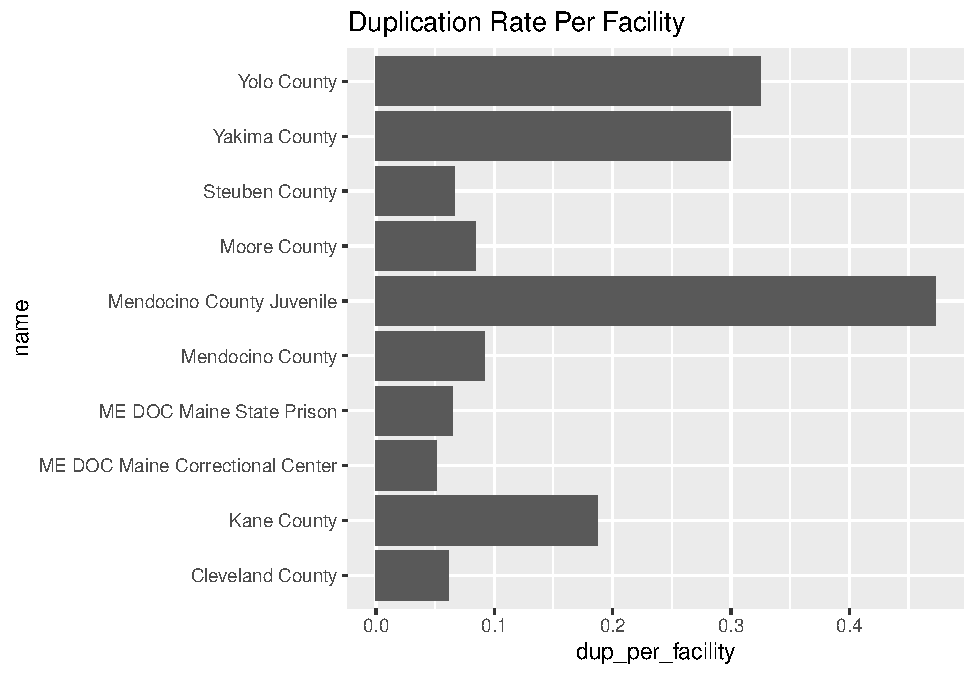
\includegraphics{report_8-5_files/figure-latex/unnamed-chunk-8-1.pdf}

Let's look at a user that has alot of fake birth dates, totally bogus
security question answers, and more.

\begin{verbatim}
## # A tibble: 58 x 29
##        id inmate_id first_name last_name hashed_password birth_date
##     <dbl> <chr>     <chr>      <chr>     <chr>           <date>    
##  1 470184 2140416   Daddy      Ortega    8d3a026cb38bf4~ 2000-02-05
##  2 472768 559       Daddy      Ortega    8d3a026cb38bf4~ 2000-05-10
##  3 473878 Papi      Daddy      Ortega    8d3a026cb38bf4~ 2001-09-08
##  4 473938 Pappy     Daddy      Ortega    8d3a026cb38bf4~ 2000-08-09
##  5 467520 214308_o~ Daddy      Ortega    8d3a026cb38bf4~ 2000-01-04
##  6 467388 00000908  Daddy      Ortega    8d3a026cb38bf4~ 2000-03-03
##  7 470208 2120416   Daddy      Ortega    8d3a026cb38bf4~ 2000-02-10
##  8 466274 22        Daddy      Ortega    8d3a026cb38bf4~ 2000-04-07
##  9 473870 Lok       Daddy      Ortega    8d3a026cb38bf4~ 2001-08-11
## 10 470461 2310804   Daddy      Ortega    8d3a026cb38bf4~ 2000-05-08
## # ... with 48 more rows, and 23 more variables: security_question_1 <chr>,
## #   security_answer_1 <chr>, security_question_2 <chr>,
## #   security_answer_2 <chr>, created_at <dttm>, updated_at <dttm>,
## #   points <dbl>, total_points <dbl>, total_spent_points <dbl>,
## #   facility_id <dbl>, status <chr>, release_date <dttm>, language <chr>,
## #   credit_balance <dbl>, balance <dbl>, desk_id <dbl>, email <chr>,
## #   phone_number <chr>, deactivation_reason <chr>, zendesk_id <chr>,
## #   state <chr>, name <chr>, goals_enabled <lgl>
\end{verbatim}

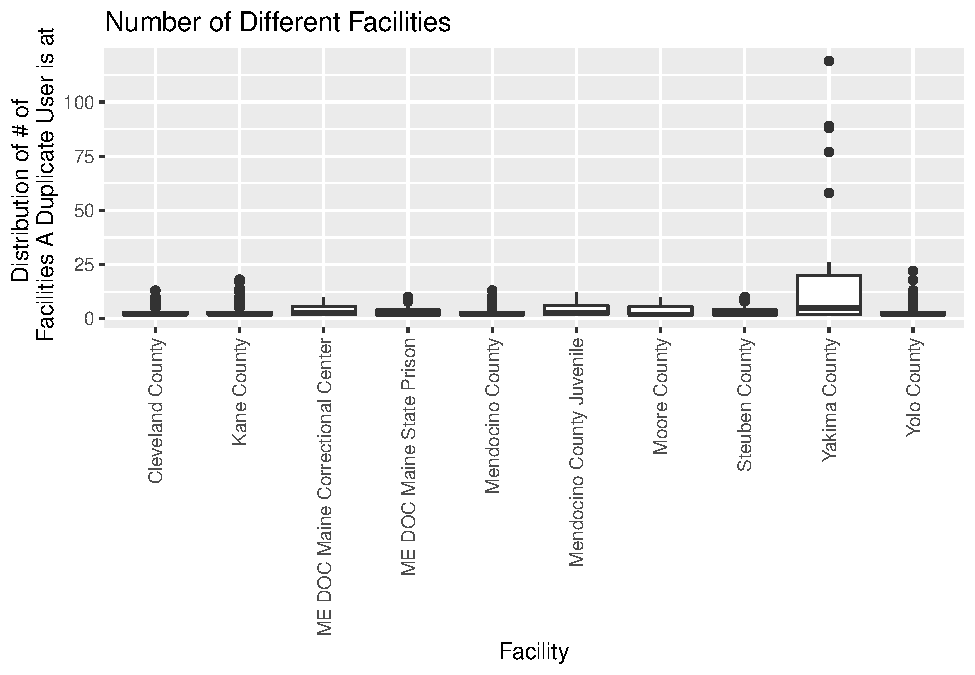
\includegraphics{report_8-5_files/figure-latex/unnamed-chunk-10-1.pdf}

\hypertarget{lets-look-at-sponsors}{%
\subsection{Let's look at sponsors}\label{lets-look-at-sponsors}}

\hypertarget{whats-the-overall-deduplication-rate-among-sponsors}{%
\subsubsection{What's the overall deduplication rate among
sponsors?}\label{whats-the-overall-deduplication-rate-among-sponsors}}

\begin{verbatim}
## # A tibble: 1 x 1
##   percent_dup
##         <dbl>
## 1       0.257
\end{verbatim}

\hypertarget{for-each-clear-duplicate-sponsor-which-ids-are-they-using}{%
\subsubsection{\texorpdfstring{For each \textbf{clear} duplicate
sponsor, which IDs are they
using?}{For each clear duplicate sponsor, which IDs are they using?}}\label{for-each-clear-duplicate-sponsor-which-ids-are-they-using}}

\begin{verbatim}
## # A tibble: 4,934 x 3
## # Groups:   first_name [2,050]
##    first_name last_name id                                                      
##    <chr>      <chr>     <chr>                                                   
##  1 A’laysha   Hernandez 76697,76697                                             
##  2 Aaliyah    Sanchez   65480,65480,82180                                       
##  3 Aaron      Leyva     88065,52417                                             
##  4 Aaron      Mascoe    90145,84330                                             
##  5 Aaron      Newson    34349,40256,90154                                       
##  6 Aaron      Pickett   53432,53432                                             
##  7 Aaron      Tardiff   89840,82829                                             
##  8 Abbagayle  Sayles    10765,10141                                             
##  9 Abbigale   Cavin     45582,45702,45612,45703,38890,38847,45519,38807,38879,4~
## 10 Abby       Bickford  67935,71998                                             
## # ... with 4,924 more rows
\end{verbatim}

\hypertarget{is-each-clear-duplicate-sponsor-using-different-emails-phone-numbers}{%
\subsection{\texorpdfstring{Is each \textbf{clear} duplicate sponsor
using different emails, phone
numbers?}{Is each clear duplicate sponsor using different emails, phone numbers?}}\label{is-each-clear-duplicate-sponsor-using-different-emails-phone-numbers}}

Yes for phone, sometimes no for emails!

\begin{verbatim}
## # A tibble: 4,934 x 3
## # Groups:   first_name [2,050]
##    first_name last_name phone_nums                                              
##    <chr>      <chr>     <chr>                                                   
##  1 A’laysha   Hernandez alayshahernandez1@icloud.com,alayshahernandez1@icloud.c~
##  2 Aaliyah    Sanchez   aaliyahsanchez9898@gmail.com,aaliyahsanchez9898@gmail.c~
##  3 Aaron      Leyva     official.kapo630@gmail.com,aaronleyva51@gmail.com       
##  4 Aaron      Mascoe    aaronryanla@gmail.com,amascoe@udel.edu                  
##  5 Aaron      Newson    aewn1281@sbcglobal.net,azo420c@gmail.com,azo4200c@gmail~
##  6 Aaron      Pickett   Kbgggg.4@gmail.com,Kbgggg.4@gmail.com                   
##  7 Aaron      Tardiff   aaron.tardiff@gmail.com,aaron.tardiff11@gmail.com       
##  8 Abbagayle  Sayles    s.abbagayle@gmail.com,brookelynnclark@gmail.com         
##  9 Abbigale   Cavin     cavinabbigale@gmail.com,abbigalecavin4@gmail.com,abbiga~
## 10 Abby       Bickford  abby.bickford1@gmail.com,Abhy.bickford1@gmail.com       
## # ... with 4,924 more rows
\end{verbatim}

\begin{verbatim}
## # A tibble: 4,934 x 3
## # Groups:   first_name [2,050]
##    first_name last_name phone_nums                                              
##    <chr>      <chr>     <chr>                                                   
##  1 A’laysha   Hernandez 19105280821,19102181648                                 
##  2 Aaliyah    Sanchez   15094159831,15092668726,18312024718                     
##  3 Aaron      Leyva     13312199654,13312625018                                 
##  4 Aaron      Mascoe    19166334682,19166622919                                 
##  5 Aaron      Newson    19165194348,12162194940,12163591165                     
##  6 Aaron      Pickett   19184299998,19189620707                                 
##  7 Aaron      Tardiff   12074584898,12072422238                                 
##  8 Abbagayle  Sayles    13098263651,13095855054                                 
##  9 Abbigale   Cavin     14054894823,14052768435,14054451396,14053531247,1405260~
## 10 Abby       Bickford  12079495135,12076056008                                 
## # ... with 4,924 more rows
\end{verbatim}

\hypertarget{baseline-network-characteristics}{%
\subsection{Baseline Network
Characteristics}\label{baseline-network-characteristics}}

\hypertarget{clustering-inmates-based-on-content-engagement}{%
\subsection{Clustering Inmates based on Content
Engagement}\label{clustering-inmates-based-on-content-engagement}}

\end{document}
